\documentclass{article}
\usepackage[utf8]{inputenc}
\usepackage[russian]{babel}
\usepackage[left=2cm,right=2cm,
top=2cm,bottom=2cm,bindingoffset=0cm]{geometry}
\usepackage{graphicx}
\usepackage{amsmath}
\usepackage{float}
\usepackage{listings}
\usepackage{url,textcomp}
\date{9 марта 2019 г.}
\author{Кондратенко Федор, гр 13632/1}
\setlength{\parindent}{0pt}
\setlength{\parskip}{5pt plus 2pt minus 1pt}
\frenchspacing
\title{Отчет по заданию №2}
\begin{document}
	\maketitle
	\section{Формулировка задания}
	Основной целью данной работы являлось моделировние бака с водой, опустошаемого в некоторые моменты времени.
	\subsection{Задачи}
	В ходе работы было необходимо смоделировать тремя разными способами наполнение бака до заданного объема. Помимо этого, требовалось разработать схему опустошения бака в случайные моменты времени.
	\section{Результаты}
	Наполнение бака было смоделировано четырьмя разными способами:
	\begin{figure}[H]
		\centering
		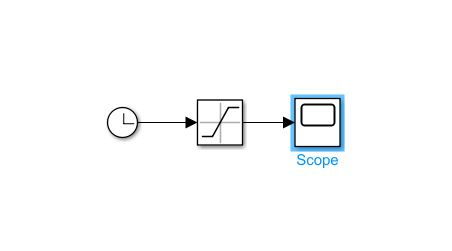
\includegraphics[width=0.7\linewidth]{model1}
		\caption{Модель 1, в качестве источника сигнала используется сигнал времени, в качестве ограничителя объема - блок saturation}
	\end{figure}
	\begin{figure}[H]
		\centering
		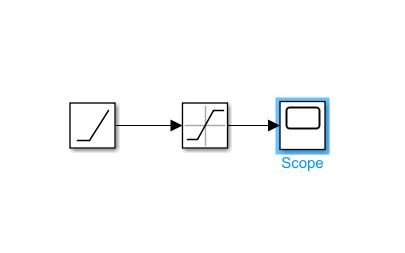
\includegraphics[width=0.7\linewidth]{model2}
		\caption{Модель 2, основным отличием от предыдущей является использование блока ramp (линейной зависимости) в качестве источника сигнала}
	\end{figure}
	\begin{figure}[H]
		\centering
		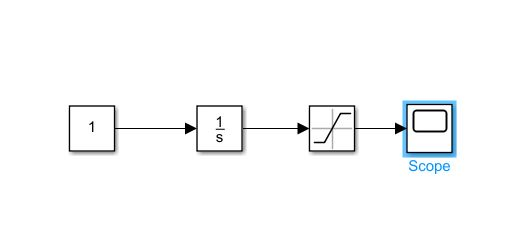
\includegraphics[width=0.7\linewidth]{model3}
		\caption{Модель 3, заполнение происходит путем задания скорости и последующим интегрированием}
	\end{figure}
	\begin{figure}[H]
		\centering
		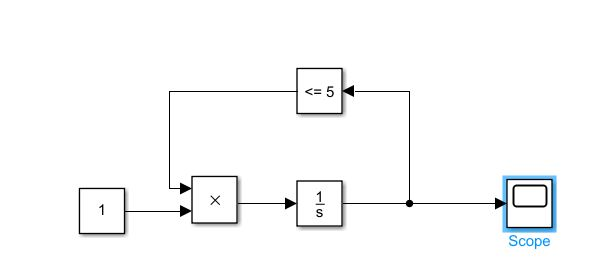
\includegraphics[width=0.7\linewidth]{model4}
		\caption{Модель 4, заполнение реализовано так же, ограничителем является сравнение текущего объема с константой}
	\end{figure}
	\begin{figure}[H]
		\centering
		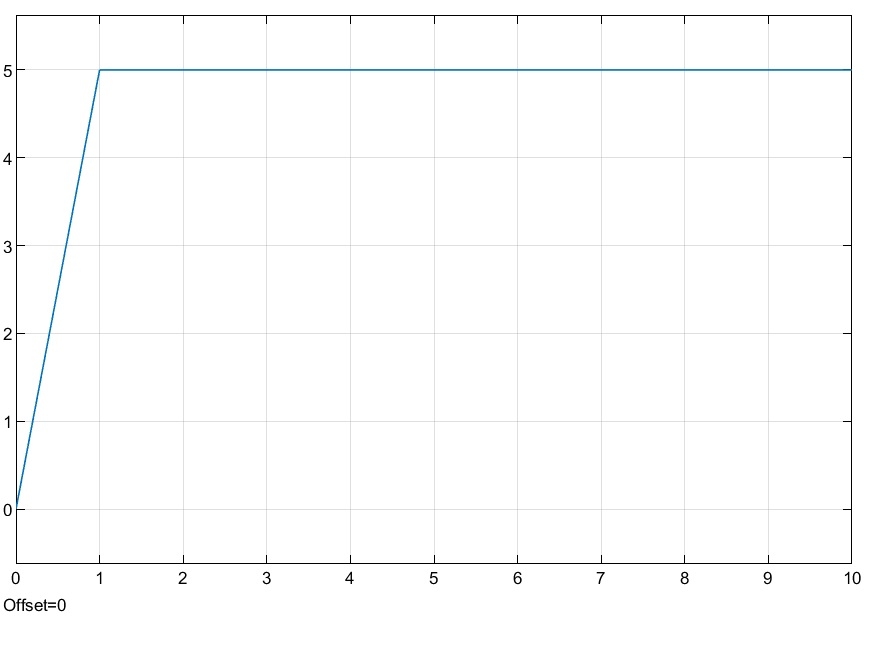
\includegraphics[width=0.7\linewidth]{Graph_1}
		\caption{График заполнения бака водой для всех моделей 1-4}
	\end{figure}
	Система слива была реализована путем вычитания из скорости слива скорости слития, вычитание производилось в случайные моменты времени.
	\begin{figure}[H]
		\centering
		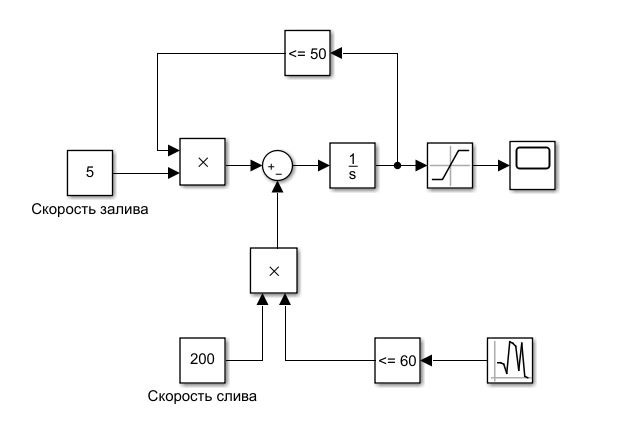
\includegraphics[width=0.7\linewidth]{model5}
		\caption{Модель 5, система слива реализована за счет сложения скоростей}
	\end{figure}
	Зависимость объема жидкости в баке от времени:
	\begin{figure}[H]
		\centering
		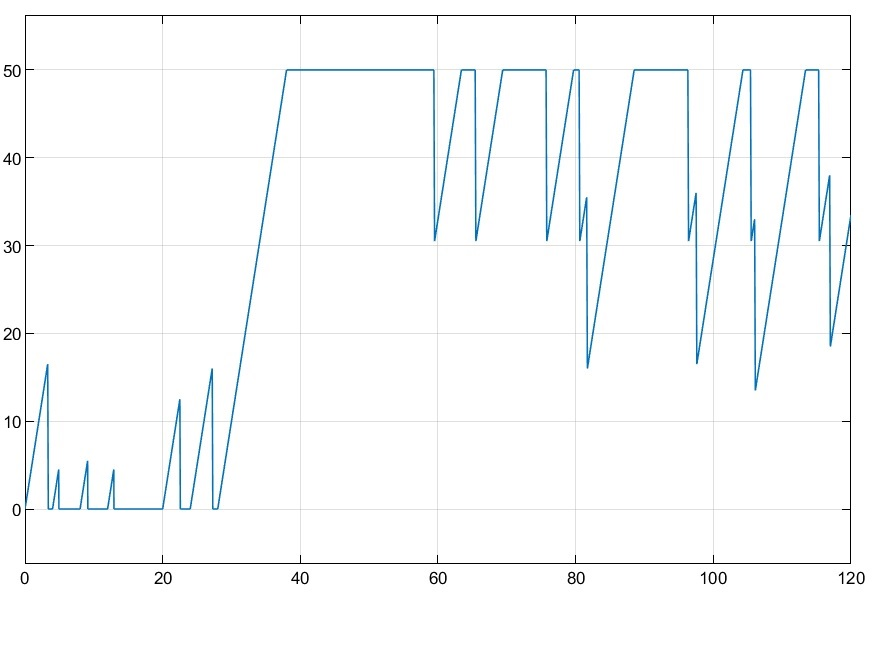
\includegraphics[width=0.7\linewidth]{Graph_2}
		\caption{Зависимость объема жидкости в баке от времени}
	\end{figure}
	
	
\end{document}